% =============================================================================
\chapter{Modelagem preditiva}\label{cap:modelagem}
% =============================================================================

Este capítulo documenta a etapa preditiva do \textit{Checkpoint}~3, implementada
em \code{src/modeling.py} e executada no notebook
\code{A3_CP3_modelagem_storytelling.ipynb}. A pergunta central é se informações
disponíveis no fechamento de um intervalo permitem antecipar algo útil sobre o
intervalo seguinte, sem que o modelo enxergue o futuro.

\section{Formulação dos problemas}\label{sec:formulacao}

Foram formulados dois problemas sobre o intervalo $t+1$, usando exclusivamente
informação disponível até o fechamento do intervalo $t$:

\begin{alineas}
  \item \textbf{tarefa A, volatilidade (regressão)}: prever a amplitude do
        intervalo seguinte e, como alvo alternativo, o retorno absoluto,
        \begin{equation}\label{eq:alvovol}
          y^{A}_t = \mathrm{amplitude}_{t+1}, \qquad
          y^{A'}_t = 10^4\,|r_{t+1}|;
        \end{equation}
  \item \textbf{tarefa B, direção (classificação binária)}: prever se o retorno
        do intervalo seguinte será positivo,
        \begin{equation}\label{eq:alvodir}
          y^{B}_t = \mathbb{I}\left(r_{t+1} > 0\right).
        \end{equation}
\end{alineas}

A tarefa A serve para calibrar limites dinâmicos de risco, o \textit{slippage}
esperado e o fatiamento TWAP ou VWAP. A tarefa B verifica se o desequilíbrio de
fluxo gera ganho direcional depois dos custos de transação. As duas tarefas
foram avaliadas em barras de 1 minuto (10.080) e de 1 segundo (604.800).

\section{Engenharia de atributos causais}\label{sec:atributos}

A função \code{build_lagged_features()} constrói os atributos a partir de cinco
defasagens, $\ell \in \{0, 1, 2, 3, 5\}$, em que $\ell = 0$ é o intervalo $t$
recém-fechado, e de três janelas móveis passadas, $w \in \{5, 15, 60\}$. Os
atributos se dividem em três famílias, combinadas em três conjuntos para um
estudo de ablação (\autoref{qua:atributos}). A lista completa dos 50 atributos
está no \autoref{apendice:atributos}.

\begin{quadro}[htbp]
\caption{\label{qua:atributos}Famílias e conjuntos de atributos dos modelos}
\begin{corpotabela}
\begin{tabularx}{\textwidth}{|L{2.6cm}|Y|C{1.9cm}|}
\hline
\textbf{Família} & \textbf{Atributos} & \textbf{Quantidade} \\ \hline
Fluxo (OFI) & $\mathrm{OFI}_{t-\ell}$ para cada defasagem; médias móveis do OFI em 5, 15 e 60 intervalos & 8 \\ \hline
Atividade & $\ln(1+\text{volume})$ e $\ln(1+\text{negócios})$ defasados; $\ln(1+\text{ticket médio})_t$; médias móveis de $\ln(1+\text{volume})$; interação $\mathrm{OFI}_t \times \ln(1+\text{volume}_t)$; nas barras de 1~s, também o indicador \code{has_trades} & 15 (16 em 1~s) \\ \hline
Volatilidade, retorno e sazonalidade & Amplitude, retorno absoluto e retorno defasados; médias móveis de amplitude e retorno absoluto e desvio-padrão móvel do retorno; razão de aceleração $\overline{\mathrm{amp}}_5 / (\overline{\mathrm{amp}}_{60} + 10^{-6})$; $\sin$ e $\cos$ da hora do dia & 27 \\ \hline
\multicolumn{3}{|l|}{\textbf{Conjuntos de ablação}: \code{apenas_ofi} (8 atributos) $\subset$ \code{fluxo_e_atividade} (23) $\subset$ \code{completo} (50; 51 em 1~s)} \\ \hline
\end{tabularx}
\end{corpotabela}
\fonteautores[Elaborado]
\end{quadro}

A sazonalidade intradiária entra por codificação cíclica, que é determinística e
portanto conhecida com antecedência, com $h_t$ igual à hora do dia em fração
(por exemplo, 14,5 para 14h30):

\begin{equation}\label{eq:sazonal}
  s_t = \sin\!\left(\frac{2\pi h_t}{24}\right), \qquad
  c_t = \cos\!\left(\frac{2\pi h_t}{24}\right).
\end{equation}

\section{Prevenção do vazamento de informação futura}\label{sec:vazamento}

Em microestrutura de alta frequência, qualquer erro sutil cria uma acurácia
artificial que desaparece em produção. O pipeline adota quatro salvaguardas:

\begin{alineas}
  \item os atributos usam apenas defasagens positivas (\code{shift(k)} com
        $k \geq 0$) e janelas móveis que terminam em $t$; nenhuma operação usa
        \code{shift(-k)} ou janelas centradas; apenas os alvos olham para
        $t+1$;
  \item as lacunas das barras de 1 segundo são preenchidas pelo último valor
        conhecido, nunca por interpolação (\autoref{sec:gaps});
  \item a padronização (\code{StandardScaler}) faz parte de um \code{Pipeline} e
        é ajustada apenas na dobra de treino;
  \item um teste de perturbação comprova a causalidade: alterar drasticamente
        todas as barras a partir de um instante (multiplicar preços, fixar o OFI
        em $-1$) não pode mudar nenhum atributo anterior a esse instante. O
        teste é executado no notebook e no conjunto de testes automatizados.
\end{alineas}

Após remover apenas as bordas incompletas (as primeiras 60 barras, exigidas pela
maior janela, e a última, que não tem alvo), restaram \textbf{10.019
observações} em 1 minuto e \textbf{604.739} em 1 segundo.

\section{Validação \textit{walk-forward}}\label{sec:validacaowf}

A validação usa dobras diárias com janela de treino expansiva
(\autoref{fig:walkforward}). Para cada dia de teste $d_k$, o conjunto de treino é
$\mathcal{T}_k = \{t : \mathrm{dia}(t) < d_k\}$ e o de teste é
$\mathcal{V}_k = \{t : \mathrm{dia}(t) = d_k\}$. Com mínimo de dois dias de
treino, há cinco dobras, que testam estritamente fora da amostra os dias 21 a
25/02 e cobrem tanto dias calmos quanto dias de estresse. As métricas são
calculadas em cada dobra e resumidas pela média simples entre as cinco.

\begin{figure}[htbp]
\caption{\label{fig:walkforward}Esquema das dobras de validação \textit{walk-forward} diária}
\begin{center}
\begin{tikzpicture}[font=\footnotesize, x=1.75cm, y=0.62cm]
  \foreach \d [count=\i from 0] in {qua 19/02, qui 20/02, sex 21/02, sáb 22/02, dom 23/02, seg 24/02, ter 25/02}{
    \node[anchor=south, font=\scriptsize] at (\i+0.5, 0.15) {\d};
  }
  \foreach \k in {1,...,5}{
    \pgfmathtruncatemacro{\teste}{\k+1}
    \node[anchor=east] at (-0.1, -\k+0.5) {Dobra \k};
    \foreach \j in {0,...,6}{
      \ifnum\j<\teste
        \fill[azulclaro, draw=azul, line width=0.4pt] (\j+0.04,-\k+0.12) rectangle (\j+0.96,-\k+0.88);
      \else\ifnum\j=\teste
        \fill[laranja!75, draw=laranja, line width=0.4pt] (\j+0.04,-\k+0.12) rectangle (\j+0.96,-\k+0.88);
      \else
        \fill[cinzaclaro, draw=cinza!60, line width=0.4pt] (\j+0.04,-\k+0.12) rectangle (\j+0.96,-\k+0.88);
      \fi\fi
    }
  }
  \fill[azulclaro, draw=azul] (0.6,-6.0) rectangle (0.9,-5.6);
  \node[anchor=west] at (0.95,-5.8) {treino};
  \fill[laranja!75, draw=laranja] (2.2,-6.0) rectangle (2.5,-5.6);
  \node[anchor=west] at (2.55,-5.8) {teste (fora da amostra)};
  \fill[cinzaclaro, draw=cinza!60] (4.6,-6.0) rectangle (4.9,-5.6);
  \node[anchor=west] at (4.95,-5.8) {não utilizado};
\end{tikzpicture}
\end{center}
\fonteautores
\end{figure}

\section{Modelos e métricas}\label{sec:modelos}

Cada tarefa compara dois \textit{baselines} ingênuos, um modelo linear e um
modelo não linear baseado em árvores (\autoref{qua:modelos}). Os
\textit{baselines} são essenciais: um modelo só tem valor se superar regras
simples que qualquer operador aplicaria sem estatística.

\begin{quadro}[htbp]
\caption{\label{qua:modelos}Modelos avaliados e seus hiperparâmetros}
\begin{corpotabela}
\begin{tabularx}{\textwidth}{|L{1.4cm}|L{4.3cm}|L{2.4cm}|Y|}
\hline
\textbf{Tarefa} & \textbf{Modelo} & \textbf{Atributos} & \textbf{Especificação} \\ \hline
\multirow{6}{=}{A (regressão)}
 & Persistência & -- & Prevê a amplitude (ou retorno absoluto) de $t+1$ igual à de $t$ \\ \cline{2-4}
 & Média móvel (15) & -- & Prevê a média dos últimos 15 intervalos \\ \cline{2-4}
 & Ridge & \code{apenas_ofi}; \code{completo} & Padronização e regressão linear com penalidade L2, $\alpha = 10$ \\ \cline{2-4}
 & \textit{HistGradientBoosting} & \code{fluxo_e_atividade}; \code{completo} & 150 iterações, profundidade 5, taxa 0,05, mínimo de 50 amostras por folha, semente 42 \\ \hline
\multirow{6}{=}{B (classifi\-cação)}
 & Classe majoritária & -- & Probabilidade constante igual à frequência de alta no treino \\ \cline{2-4}
 & Persistência de sinal & -- & Prevê alta se o retorno de $t$ foi positivo (probabilidade 0,99 ou 0,01) \\ \cline{2-4}
 & Regressão logística & \code{apenas_ofi}; \code{completo} & Padronização e penalidade L2 com $C = 0,5$, até 500 iterações \\ \cline{2-4}
 & \textit{HistGradientBoosting} & \code{fluxo_e_atividade}; \code{completo} & Mesmos hiperparâmetros da tarefa A \\ \hline
\end{tabularx}
\end{corpotabela}
\fonteautores[Elaborado]
\end{quadro}

Na tarefa A, as previsões negativas são truncadas em zero. As métricas de
regressão são o erro absoluto médio (MAE), a raiz do erro quadrático médio
(RMSE), o coeficiente de determinação fora da amostra e a correlação de postos
de Spearman entre previsto e realizado:

\begin{equation}\label{eq:metricasreg}
  \mathrm{MAE} = \frac{1}{n}\sum_{t}|y_t - \hat{y}_t|, \qquad
  \mathrm{RMSE} = \sqrt{\frac{1}{n}\sum_{t}(y_t - \hat{y}_t)^2}, \qquad
  R^2 = 1 - \frac{\sum_t (y_t - \hat{y}_t)^2}{\sum_t (y_t - \bar{y})^2}.
\end{equation}

\noindent Fora da amostra, $R^2$ pode ser negativo, o que indica um modelo pior
que prever a média do próprio dia de teste. Na tarefa B, além de acurácia,
acurácia balanceada, ROC-AUC e perda logarítmica, mede-se o \textbf{retorno
bruto} de uma estratégia que compra quando $\hat{p}_t \geq 0,5$ e vende caso
contrário,

\begin{equation}\label{eq:retornobruto}
  \bar{g} = \frac{1}{n}\sum_{t} s_t \cdot 10^4\, r_{t+1}, \qquad
  s_t = \begin{cases} +1, & \hat{p}_t \geq 0,5,\\ -1, & \hat{p}_t < 0,5, \end{cases}
\end{equation}

\noindent e o mesmo retorno restrito aos 10\,\% de sinais mais confiantes, isto
é, aos intervalos em que $|\hat{p}_t - 0,5|$ está acima do seu percentil 90. O
retorno bruto não desconta taxas; ele é comparado depois aos custos de execução.

\section{Resultados em barras de 1 minuto}\label{sec:resultados1m}

\subsection{Volatilidade}\label{sec:vol1m}

\begin{table}[htbp]
\caption{\label{tab:vol1m}Previsão da amplitude do minuto seguinte: médias das cinco dobras}
\begin{corpotabela}
\begin{tabular}{llrrrr}
\toprule
Modelo & Família & MAE (bps) & RMSE (bps) & $R^2$ & Spearman \\
\midrule
Persistência & \textit{baseline} & 3,296 & 4,871 & 0,074 & 0,530 \\
Média móvel (15) & \textit{baseline} & 2,775 & 4,154 & 0,353 & 0,603 \\
Ridge (apenas OFI) & linear & 5,297 & 7,265 & $-0,963$ & 0,044 \\
\textbf{Ridge (completo)} & linear & \textbf{2,668} & \textbf{3,999} & \textbf{0,385} & \textbf{0,616} \\
HGB (fluxo e atividade) & não linear & 2,924 & 4,414 & 0,301 & 0,583 \\
HGB (completo) & não linear & 2,835 & 4,320 & 0,314 & 0,574 \\
\bottomrule
\end{tabular}
\end{corpotabela}
\fonte{Elaborada pelos autores (2026), com dados de \citeonline{glitchlist2026}. HGB: \textit{HistGradientBoosting}.}
\end{table}

A \autoref{tab:vol1m} mostra que a volatilidade do minuto seguinte é previsível.
O Ridge com todos os atributos teve o melhor desempenho em todas as métricas
($R^2 = 0,385$, Spearman de 0,616), superando a média móvel de 15 minutos, que
já é um \textit{baseline} forte ($R^2 = 0,353$). O OFI sozinho não prevê
volatilidade ($R^2 < 0$), o que é coerente com a matriz de correlação da
\autoref{fig:spearman}. Os modelos de árvore ficaram atrás do Ridge porque não
extrapolam: suas previsões ficam limitadas aos valores vistos no treino, e o
pânico de 25/02 produziu amplitudes acima de tudo o que havia nos dias
anteriores. O painel direito da \autoref{fig:modvol} ilustra esse efeito.

\begin{figure}[htbp]
\caption{\label{fig:modvol}Desempenho na previsão de volatilidade e série prevista em 25/02}
\begin{center}
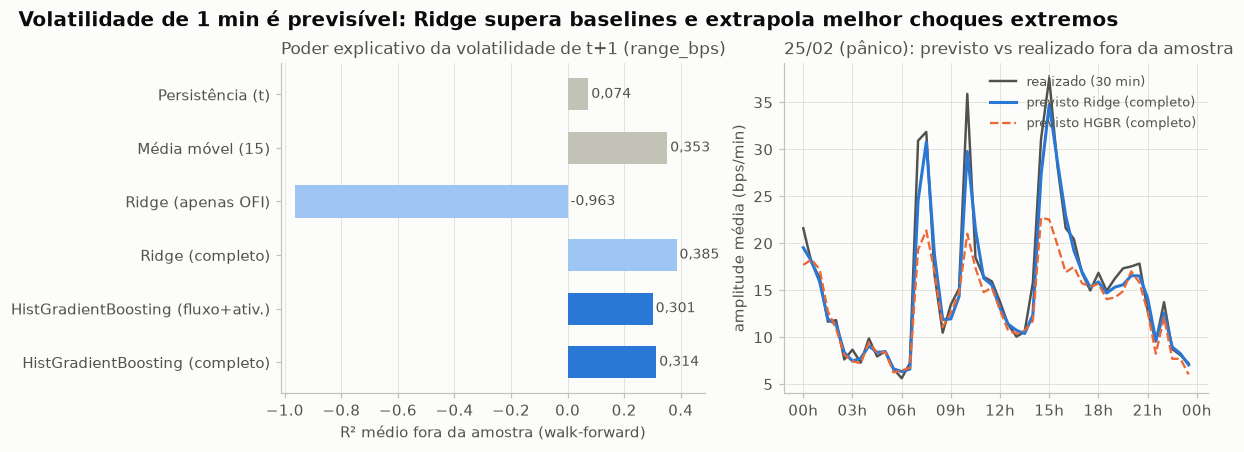
\includegraphics[width=\textwidth]{figuras/fig_modelo_volatilidade.png}
\end{center}
\fontedados
\end{figure}

Com o alvo alternativo, o retorno absoluto do minuto seguinte, o padrão se repete
em nível mais baixo, porque o retorno absoluto é uma medida mais ruidosa que a
amplitude: Ridge (completo) obteve $R^2 = 0,154$ e Spearman de 0,370, contra
$R^2 = 0,146$ da média móvel e $R^2 = -0,482$ da persistência.

\subsection{Direção do retorno}\label{sec:dir1m}

\begin{table}[htbp]
\caption{\label{tab:dir1m}Previsão da direção do minuto seguinte: médias das cinco dobras}
\begin{corpotabela}
\setlength{\tabcolsep}{4pt}
\begin{tabularx}{\textwidth}{L{3.6cm}RRRRRR}
\toprule
Modelo & Acurácia & Acur. balanc. & ROC-AUC & Perda log. & Ret. bruto (bps) & Ret. top 10\,\% (bps) \\
\midrule
Classe majoritária & 0,510 & 0,500 & 0,500 & 0,693 & 0,091 & 0,091 \\
Persistência de sinal & 0,530 & 0,529 & 0,529 & 2,172 & 0,257 & 0,257 \\
\textbf{Logit (apenas OFI)} & 0,526 & 0,524 & \textbf{0,536} & \textbf{0,691} & 0,155 & \textbf{0,360} \\
Logit (completo) & 0,517 & 0,516 & 0,523 & 0,699 & $-0,004$ & $-0,178$ \\
HGB (fluxo e atividade) & 0,520 & 0,520 & 0,521 & 0,705 & 0,172 & 0,330 \\
HGB (completo) & 0,511 & 0,511 & 0,513 & 0,709 & 0,015 & $-0,119$ \\
\bottomrule
\end{tabularx}
\end{corpotabela}
\fonte{Elaborada pelos autores (2026), com dados de \citeonline{glitchlist2026}. A perda logarítmica alta da persistência decorre das probabilidades extremas (0,01 e 0,99).}
\end{table}

A direção do minuto seguinte fica próxima do acaso (\autoref{tab:dir1m}). O
melhor ROC-AUC, de 0,536, é da regressão logística apenas com OFI, e o melhor
retorno bruto nos 10\,\% de sinais mais confiantes é de $+0,36$~bps por operação.
Acrescentar atributos piorou o resultado fora da amostra, sinal de que os modelos
mais ricos aprendem ruído. A \autoref{fig:moddir} compara esses ganhos com os
custos de execução.

\begin{figure}[htbp]
\caption{\label{fig:moddir}Discriminação direcional e retorno bruto contra o custo de transação}
\begin{center}
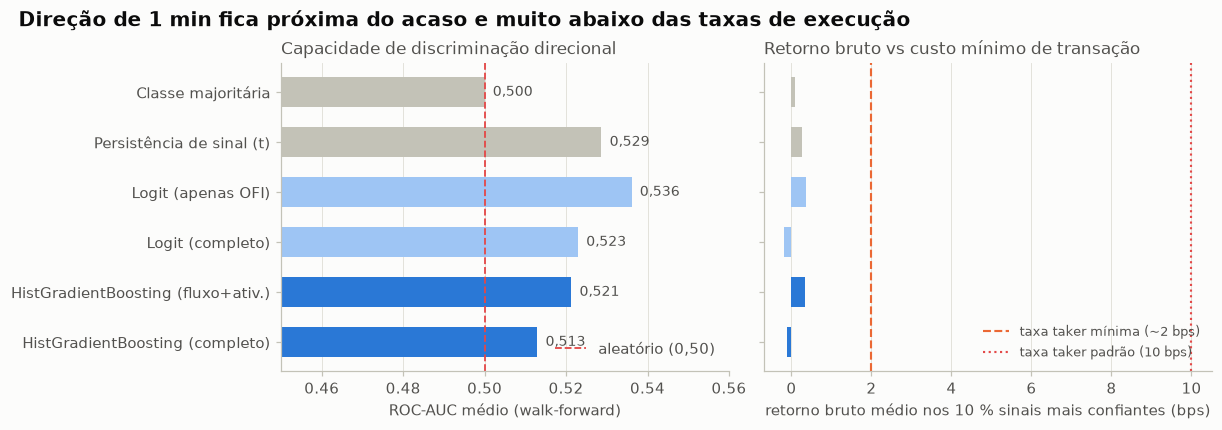
\includegraphics[width=\textwidth]{figuras/fig_modelo_direcao.png}
\end{center}
\fontedados
\end{figure}

\section{Resultados em barras de 1 segundo}\label{sec:resultados1s}

No \textit{Checkpoint}~2, levantou-se a hipótese de que o poder preditivo do
fluxo pudesse aparecer em escalas menores que 1 minuto. O mesmo pipeline causal
e \textit{walk-forward} foi aplicado às 604.800 barras de 1 segundo. Na
classificação, foram avaliados apenas os segundos em que o preço variou
($r_{t+1} \neq 0$), para evitar que segundos ``planos'' inflassem a acurácia.

\begin{table}[htbp]
\caption{\label{tab:vol1s}Previsão da amplitude do segundo seguinte: médias das cinco dobras}
\begin{corpotabela}
\begin{tabular}{llrrrr}
\toprule
Modelo & Família & MAE (bps) & RMSE (bps) & $R^2$ & Spearman \\
\midrule
Persistência & \textit{baseline} & 0,341 & 0,719 & $-0,465$ & 0,352 \\
Média móvel (15) & \textit{baseline} & 0,306 & 0,556 & 0,121 & 0,380 \\
Ridge (apenas OFI) & linear & 0,369 & 0,666 & $-0,149$ & 0,100 \\
\textbf{Ridge (completo)} & linear & \textbf{0,302} & \textbf{0,543} & \textbf{0,164} & 0,427 \\
HGB (fluxo e atividade) & não linear & 0,312 & 0,560 & 0,126 & \textbf{0,434} \\
HGB (completo) & não linear & 0,306 & 0,550 & 0,150 & 0,430 \\
\bottomrule
\end{tabular}
\end{corpotabela}
\fontedados
\end{table}

\begin{table}[htbp]
\caption{\label{tab:dir1s}Previsão da direção do segundo seguinte, apenas segundos com variação de preço}
\begin{corpotabela}
\setlength{\tabcolsep}{4pt}
\begin{tabularx}{\textwidth}{L{3.6cm}RRRRRR}
\toprule
Modelo & Acurácia & Acur. balanc. & ROC-AUC & Perda log. & Ret. bruto (bps) & Ret. top 10\,\% (bps) \\
\midrule
Classe majoritária & 0,503 & 0,500 & 0,500 & 0,693 & $-0,004$ & $-0,004$ \\
Persistência de sinal & 0,456 & 0,457 & 0,457 & 2,511 & 0,117 & 0,117 \\
Logit (apenas OFI) & 0,549 & 0,549 & 0,582 & 0,685 & $-0,096$ & $-0,106$ \\
Logit (completo) & 0,635 & 0,635 & 0,695 & 0,633 & 0,082 & 0,135 \\
HGB (fluxo e atividade) & 0,676 & 0,676 & 0,754 & 0,573 & 0,105 & 0,061 \\
\textbf{HGB (completo)} & \textbf{0,781} & \textbf{0,781} & \textbf{0,837} & \textbf{0,470} & 0,106 & 0,054 \\
\bottomrule
\end{tabularx}
\end{corpotabela}
\fontedados
\end{table}

Em volatilidade (\autoref{tab:vol1s}), os modelos com todos os atributos voltam a
superar os \textit{baselines}, com Spearman em torno de 0,43 contra 0,35 da
persistência. Em direção (\autoref{tab:dir1s}), o resultado parece
surpreendente: o \textit{HistGradientBoosting} com todos os atributos acerta
78,1\,\% das direções, com ROC-AUC de 0,837. A explicação está na própria tabela:
a persistência de sinal acerta só 45,6\,\%, ou seja, em 54,4\,\% dos casos o
segundo seguinte \textbf{reverte} o anterior. É o \textit{bid-ask bounce}
descrito por \citeonline{roll1984}: o último preço oscila entre a melhor
oferta de compra e a de venda conforme o lado do agressor, e o modelo aprende a
prever esse rebote de um \textit{tick}. Como o movimento previsto é minúsculo, o
retorno bruto médio é de apenas $+0,11$~bps por operação ($+0,05$~bps nos sinais
mais confiantes).

\section{Viabilidade operacional}\label{sec:viabilidade}

A taxa \textit{taker} da Binance no mercado à vista varia, conforme o nível do
cliente, de cerca de 2 a 10~bps por perna \cite{binancefees}; uma operação
completa paga duas pernas, além do \textit{slippage}. O \autoref{qua:viabilidade}
confronta os resultados com esses custos.

\begin{quadro}[htbp]
\caption{\label{qua:viabilidade}Viabilidade operacional dos sinais para a mesa de execução}
\begin{corpotabela}
\begin{tabularx}{\textwidth}{|L{2.6cm}|Y|L{4.4cm}|}
\hline
\textbf{Dimensão} & \textbf{Evidência em 1 minuto e 1 segundo} & \textbf{Veredito} \\ \hline
Previsão de volatilidade & Em 1~min, Ridge (completo) atinge $R^2 = 0,385$ e Spearman de 0,616, acima da média móvel de 15 minutos ($R^2 = 0,353$) e dos modelos de árvore. Em 1~s, Ridge e HGB atingem Spearman de cerca de 0,43. O OFI sozinho não prevê volatilidade. & \textbf{Viável e recomendada}: usar a previsão do Ridge para calibrar limites dinâmicos de \textit{slippage}, alertas e o ritmo do fatiamento TWAP ou VWAP. \\ \hline
Previsão de direção & Em 1~min, o melhor ROC-AUC é de 0,536, com retorno bruto de $+0,36$~bps nos sinais mais confiantes. Em 1~s, a acurácia de 78,1\,\% captura o \textit{bid-ask bounce}, com retorno bruto de $+0,11$~bps. & \textbf{Inviável para operar direção}: o ganho bruto, abaixo de 0,4~bps, é muito menor que o custo de 2 a 10~bps por perna. Útil apenas como filtro passivo de \textit{timing}. \\ \hline
\end{tabularx}
\end{corpotabela}
\fonteautores[Elaborado]
\end{quadro}

O resultado confirma a hipótese formulada para a pergunta P3: o fluxo agressor
explica o preço no instante em que ocorre, mas não gera previsão direcional
lucrativa, o que é consistente com a eficiência de mercado nessa escala
\cite{fama1970}. Por outro lado, a volatilidade tem persistência e sazonalidade
suficientes para ser prevista, e é essa previsão que tem valor prático imediato
para a mesa.
